\section{Borsuk-Ulam 定理}
\label{section:ch09-sec57}

这里有一个费尽心思才能得到解答的问题. 假设在平面 $\mathbb{R}^{2}$ 上给定了一个有界的多边形区域 $A$. 不管 $A$ 的形状如何, 容易证明总存在一条直线将 $A$ 平分, 也就是说把 $A$ 切割成面积相等的两部分. 为此, 取水平线 $y=c$, 用 $f(c)$ 表示 $A$ 在这条直线下面部分的面积, 由于 $f(c)$ 是 $c$ 的连续函数, 用介值定理便能发现有一个 $c$ 使得 $f(c)$ 恰好等于 $A$ 的面积的一半.

现在假定给定了两个区域 $A_1$ 和 $A_2$, 并且要求用一条直线同时将这两部分平分. 即使是有这条直线找起来也肯定不容易. 不相信的话, 你可以试试用一条直线平分两个三角形.

事实上, 这条直线总是存在的. 这个结论是下面介绍的著名的 Borsuk-Ulam 定理的一个推论.

\begin{definition}[对径点与保持对径点的映射]
\label{definition:ch09-sec57-antipode}
$S^{n}$ 中的点 $x$ 的\textbf{对径点}(antipode) 是点 $-x$. 映射 $h\colon S^{n}\to S^{m}$ 称为\textbf{保持对径点的}(antipode-preserving), 如果对于所有 $x\in S^{n}$, 有 $h(-x)=-h(x)$.
\end{definition}

\begin{theorem}
\label{theorem:ch09-sec57-57-1}
如果 $h\colon S^{1}\to S^{1}$ 是保持对径点的连续映射, 则 $h$ 不是零伦的.
\end{theorem}

\begin{proof}
记 $b_0$ 为 $S^{1}$ 中的点 $(1,0)$. 设 $\rho\colon S^{1}\to S^{1}$ 为 $S^{1}$ 的一个旋转, 将 $h(b_0)$ 映到 $b_0$. 因为 $\rho$ 保持对径点, 所以 $\rho\circ h$ 也保持对径点. 假若 $H$ 是 $h$ 与某常值映射之间的同伦, 那么 $\rho\circ H$ 便是 $\rho\circ h$ 与某常值映射之间的同伦. 因此, 只要证明加上附加条件 $h(b_0)=b_0$ 之后这个定理成立即可.

\textbf{第一步.} 设 $q\colon S^{1}\to S^{1}$ 定义为 $q(z)=z^2$, 其中 $z$ 是一个复数. 如果用实坐标表示, 这个映射便是 $q(\cos\theta,\sin\theta)=(\cos 2\theta,\sin 2\theta)$. 由于映射 $q$ 是连续的、闭的和满的, 所以它是一个商映射. $S^{1}$ 中的任何一个点在映射 $q$ 下的原像是 $S^{1}$ 中的一对对径点 $z$ 和 $-z$. 由于 $h(-z)=-h(z)$, 我们有等式 $q(h(-z))=q(h(z))$. 因此, 由于 $q$ 是一个商映射, 映射 $q\circ h$ 诱导出一个连续映射 $k\colon S^{1}\to S^{1}$ 使得 $k\circ q=q\circ h$.
\[
\begin{array}{ccc}
S^{1} & \xrightarrow{h} & S^{1}\\
{\scriptstyle q}\downarrow & & \downarrow{\scriptstyle q}\\
S^{1} & \xrightarrow{k} & S^{1}
\end{array}
\]
我们有 $q(b_0)=h(b_0)=b_0$, 所以 $k(b_0)=b_0$. 此外, $h(-b_0)=-b_0$.

\textbf{第二步.} 我们证明 $\pi_1(S^{1},b_0)$ 到自身的同态 $k_*$ 是非平凡的.

为此, 我们首先指出 $q$ 是一个覆叠映射. (这曾在第 53 节的习题中给出.) 其证明类似于标准映射 $p\colon\mathbb{R}\to S^{1}$ 是覆叠映射的证明. 例如, 如果 $U$ 是 $S^{1}$ 中由第二个坐标为正数组成的子集, 则 $p^{-1}(U)$ 由 $S^{1}$ 中在 $\mathbb{R}^{2}$ 的第一象限和第三象限的点构成. 映射 $q$ 将这两个集合的每一个同胚地映射到 $U$ 上. 如果 $U$ 是 $S^{1}$ 与下半开平面、右半开平面或左半开平面的交, 类似的论断也是成立的.

其次, 注意如果 $\tilde{f}$ 是 $S^{1}$ 中的一条从 $b_0$ 到 $-b_0$ 的道路, 则回路 $f=q\circ\tilde{f}$ 代表 $\pi_1(S^{1},b_0)$ 中的一个非平凡的元素. 因为 $\tilde{f}$ 是 $f$ 在 $S^{1}$ 中的一个提升, 它开始于 $b_0$ 但不终结于 $b_0$.

最后我们指出 $k_*$ 是非平凡的. 设 $\tilde{f}$ 是 $S^{1}$ 中从 $b_0$ 到 $-b_0$ 的一条道路, $f$ 是回路 $q\circ\tilde{f}$, 则 $k_*[f]$ 是非平凡的, 因为 $k_*[f]=[k\circ(q\circ\tilde{f})]=[q\circ(h\circ\tilde{f})]$, 后者非平凡是因为 $h\circ\tilde{f}$ 是 $S^{1}$ 中从 $b_0$ 到 $-b_0$ 的一条道路.

\textbf{第三步.} 最后证明同态 $h_*$ 是非平凡的, 所以 $h$ 不是零伦的.

同态 $k_*$ 是单射, 因为它是一个无限循环群到自身的非平凡同态. 同态 $q_*$ 也是单射, 实际上 $q_*$ 相当于整数群乘 $2$ 的那个同态. 这导致 $k_*\circ q_*$ 是单射. 由于 $q_*\circ h_*=k_*\circ q_*$, 同态 $h_*$ 也应当是单射.
\end{proof}

\par
\begin{figure}[htbp]
\centering
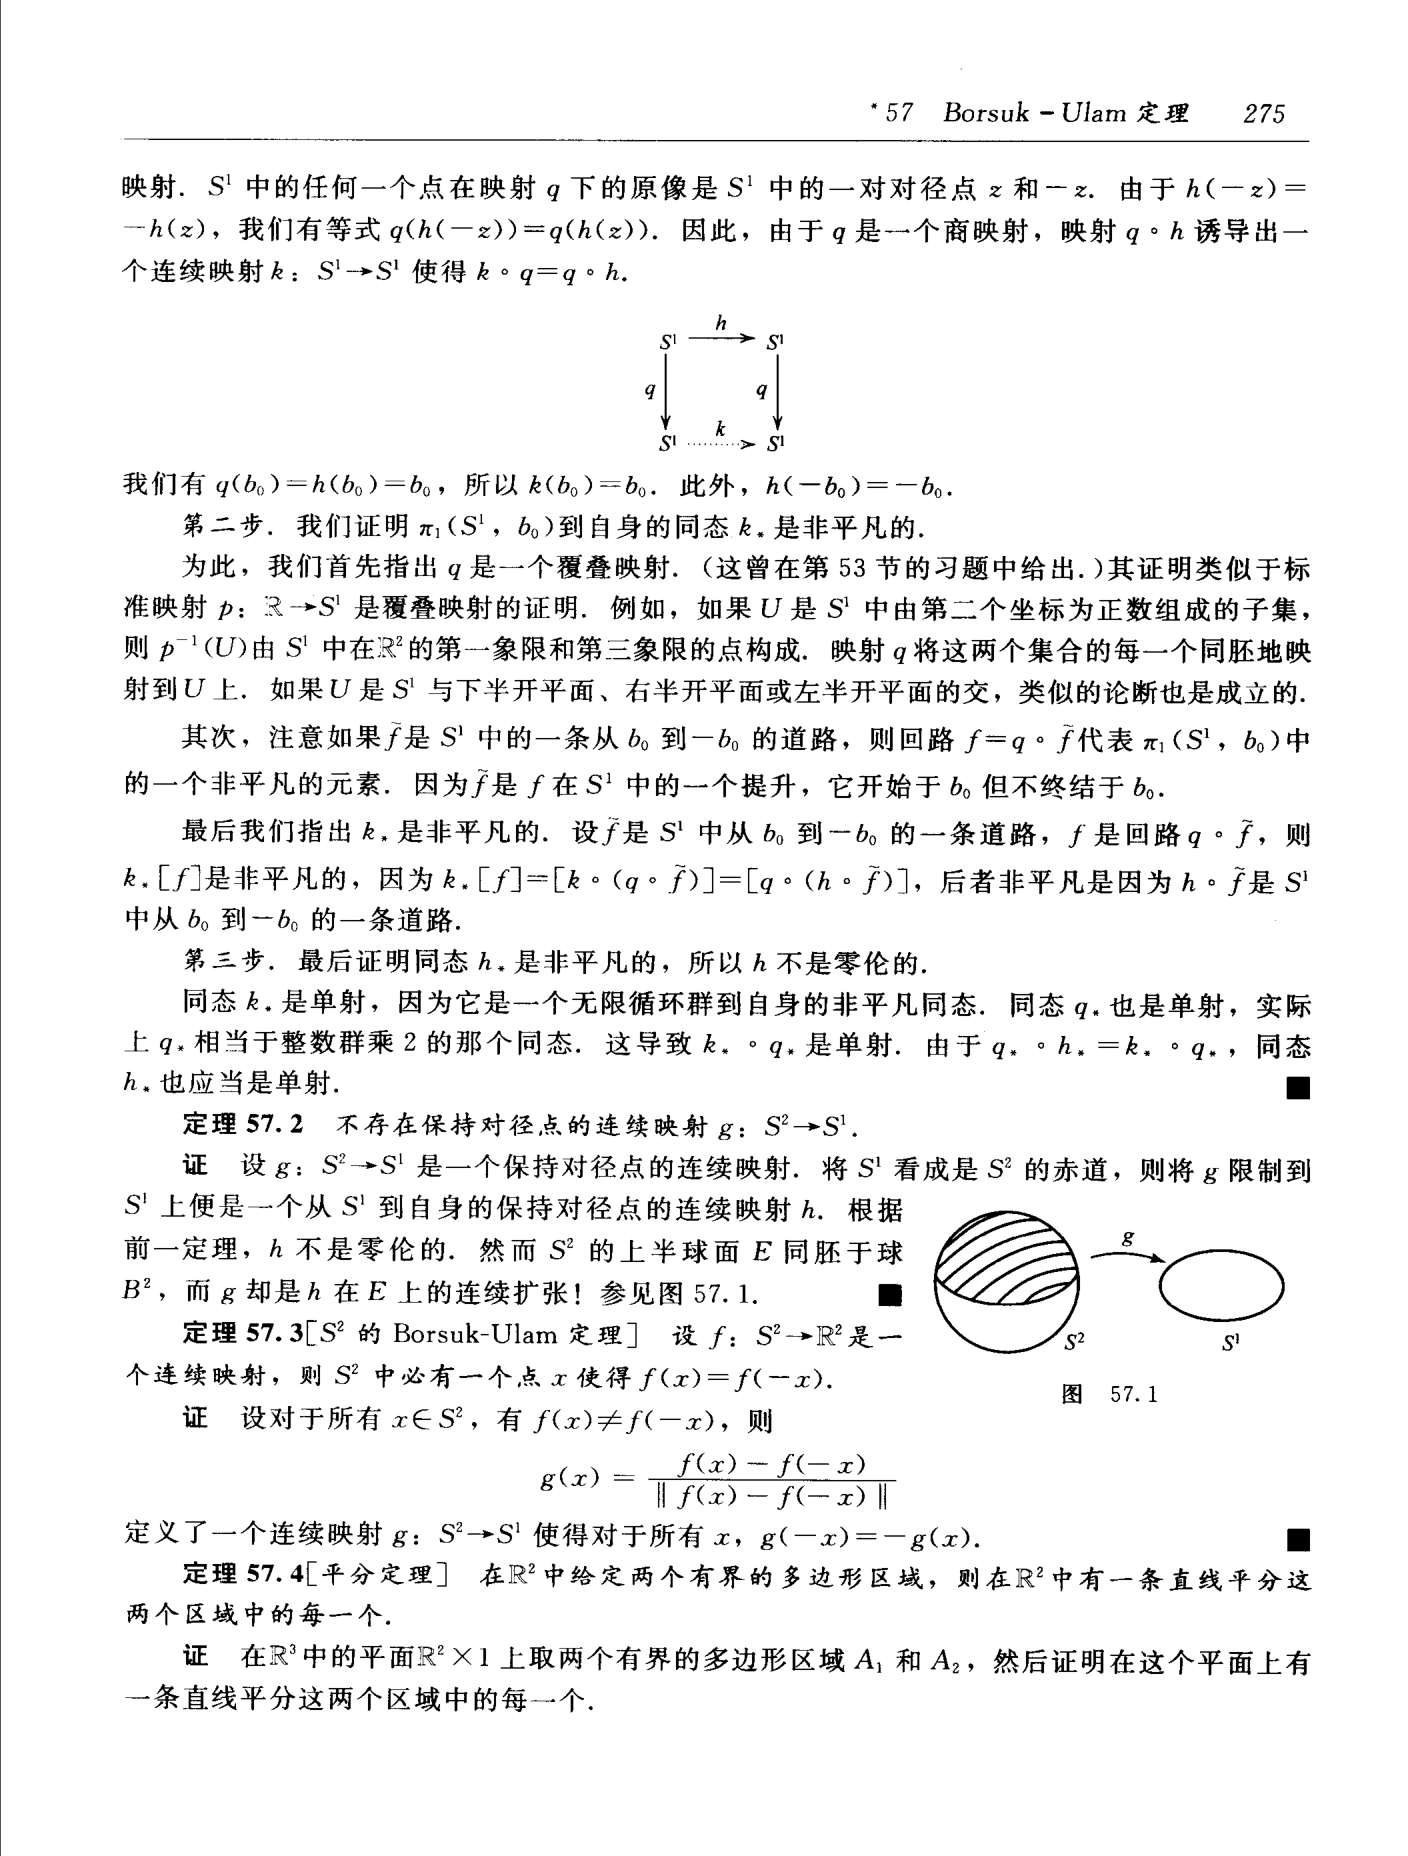
\includegraphics[width=0.5\textwidth]{image/fig-57-1.png}
\caption{定理 \cref{theorem:ch09-sec57-57-2}.}
\label{figure:ch09-fig-57-1}
\end{figure}

\par
\begin{figure}[htbp]
\centering
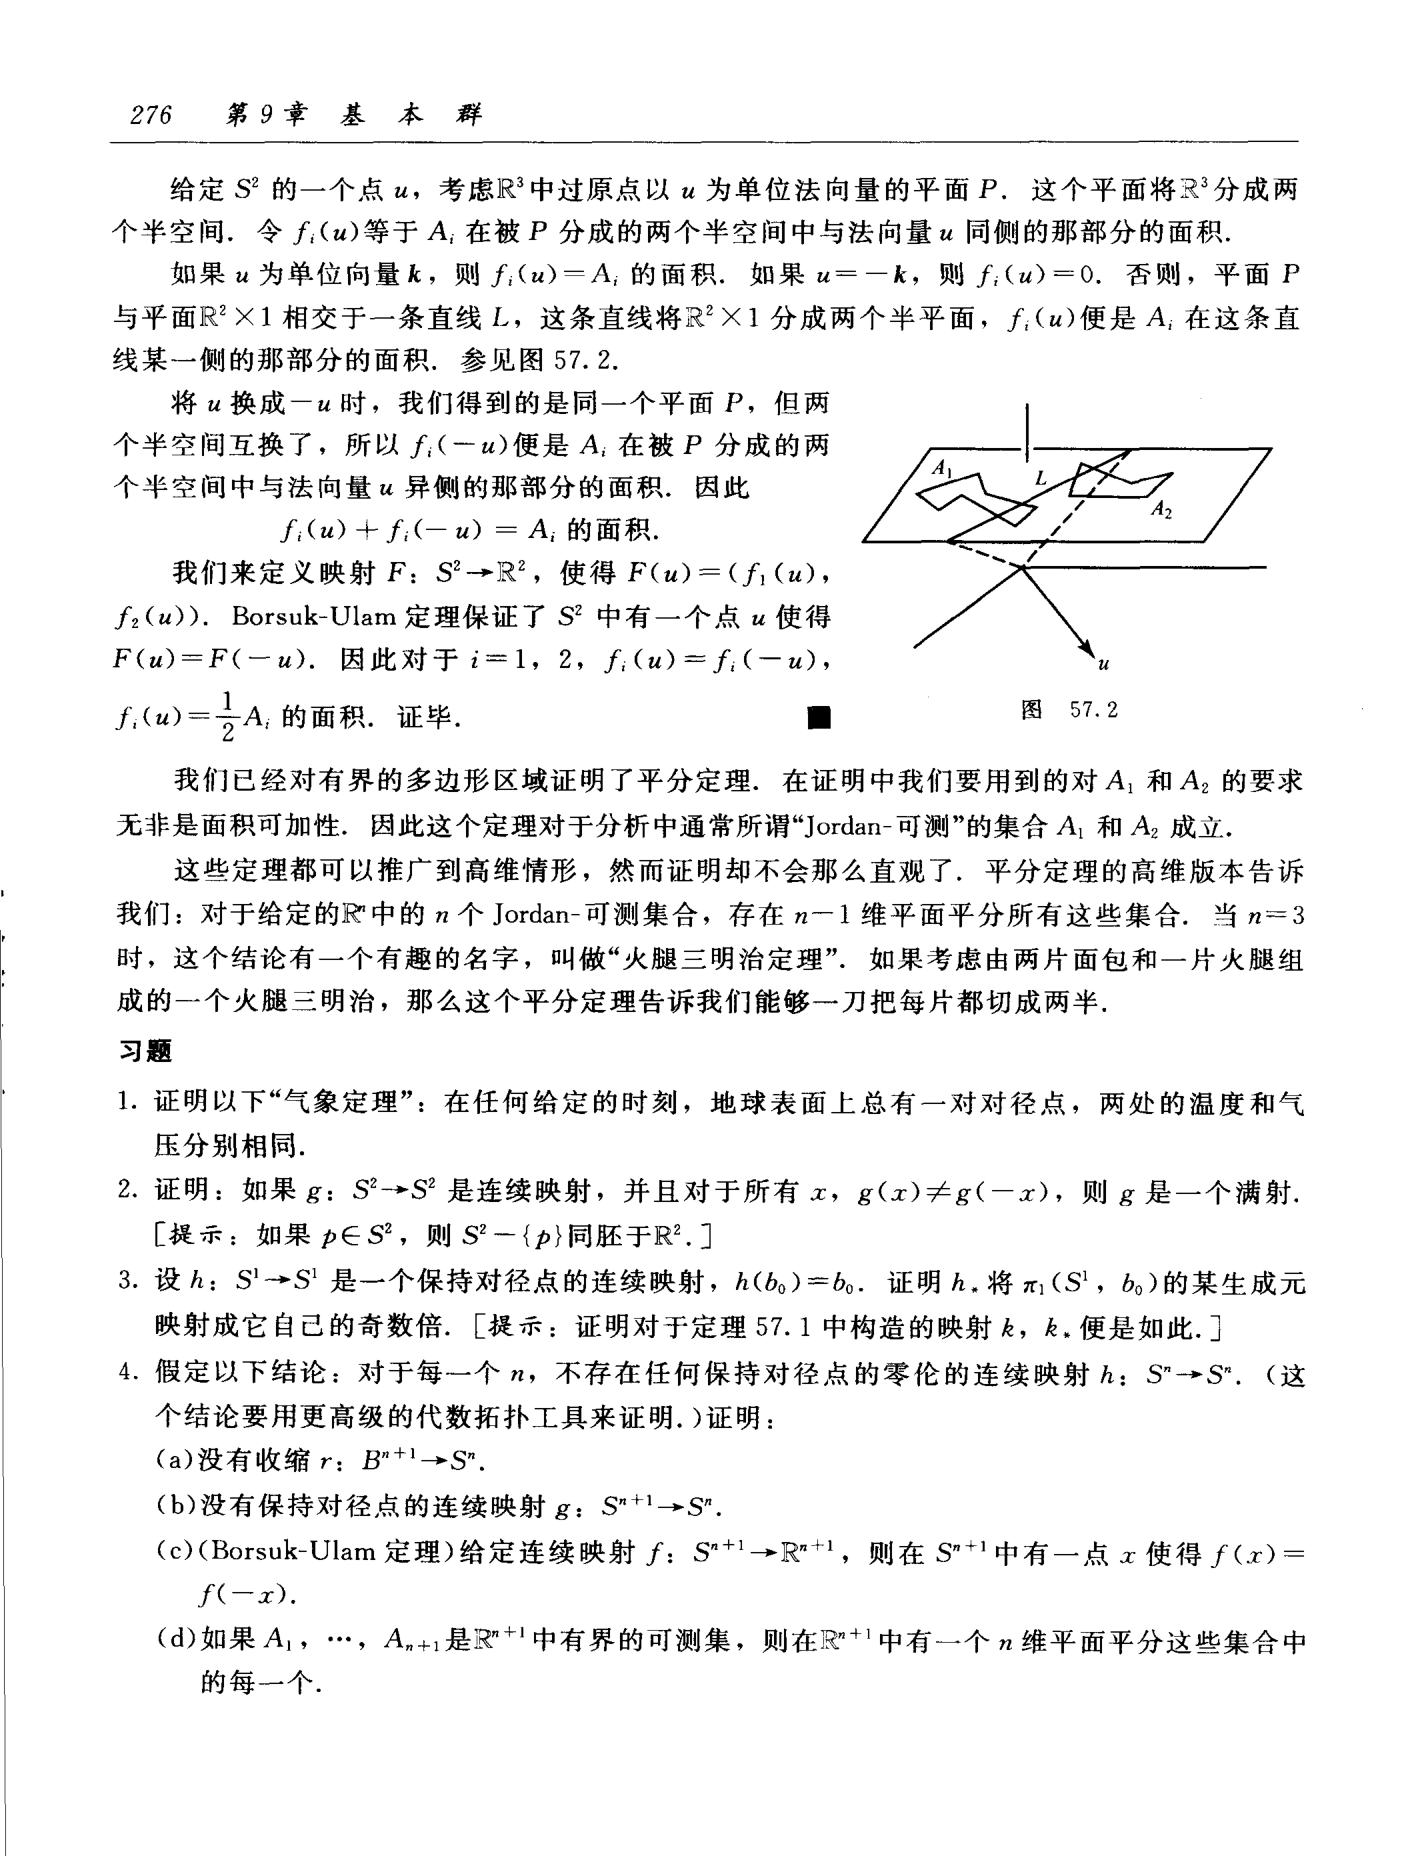
\includegraphics[width=0.5\textwidth]{image/fig-57-2.png}
\caption{平分定理.}
\label{figure:ch09-fig-57-2}
\end{figure}

\begin{theorem}
\label{theorem:ch09-sec57-57-2}
不存在保持对径点的连续映射 $g\colon S^{2}\to S^{1}$.
\end{theorem}

\begin{proof}
设 $g\colon S^{2}\to S^{1}$ 是一个保持对径点的连续映射. 将 $S^{1}$ 看成是 $S^{2}$ 的赤道, 则将 $g$ 限制到 $S^{1}$ 上便是一个从 $S^{1}$ 到自身的保持对径点的连续映射 $h$. 根据前一定理, $h$ 不是零伦的. 然而 $S^{2}$ 的上半球面 $E$ 同胚于球 $B^{2}$, 而 $g$ 却是 $h$ 在 $E$ 上的连续扩张! 参见图 \cref{figure:ch09-fig-57-1}.
\end{proof}


\begin{theorem}[$S^{2}$ 的 Borsuk-Ulam 定理]
\label{theorem:ch09-sec57-57-3}
设 $f\colon S^{2}\to\mathbb{R}^{2}$ 是一个连续映射, 则 $S^{2}$ 中必有一个点 $x$ 使得 $f(x)=f(-x)$.
\end{theorem}

\begin{proof}
设对于所有 $x\in S^{2}$, 有 $f(x)\neq f(-x)$, 则
\[
g(x)=\frac{f(x)-f(-x)}{\|f(x)-f(-x)\|}
\]
定义了一个连续映射 $g\colon S^{2}\to S^{1}$ 使得对于所有 $x$, $g(-x)=-g(x)$.
\end{proof}

\begin{theorem}[平分定理]
\label{theorem:ch09-sec57-57-4}
在 $\mathbb{R}^{2}$ 中给定两个有界的多边形区域, 则在 $\mathbb{R}^{2}$ 中有一条直线平分这两个区域中的每一个.
\end{theorem}

\begin{proof}
在 $\mathbb{R}^{3}$ 中的平面 $\mathbb{R}^{2}\times 1$ 上取两个有界的多边形区域 $A_1$ 和 $A_2$, 然后证明在这个平面上有一条直线平分这两个区域中的每一个.

给定 $S^{2}$ 的一个点 $u$, 考虑 $\mathbb{R}^{3}$ 中过原点以 $u$ 为单位法向量的平面 $P$. 这个平面将 $\mathbb{R}^{3}$ 分成两个半空间. 令 $f_i(u)$ 等于 $A_i$ 在被 $P$ 分成的两个半空间中与法向量 $u$ 同侧的那部分的面积.

如果 $u$ 为单位向量 $\boldsymbol{k}$, 则 $f_i(u)=A_i$ 的面积. 如果 $u=-\boldsymbol{k}$, 则 $f_i(u)=0$. 否则, 平面 $P$ 与平面 $\mathbb{R}^{2}\times 1$ 相交于一条直线 $L$, 这条直线将 $\mathbb{R}^{2}\times 1$ 分成两个半平面, $f_i(u)$ 便是 $A_i$ 在这条直线某一侧的那部分的面积. 参见图 \cref{figure:ch09-fig-57-2}.

将 $u$ 换成 $-u$ 时, 我们得到的是同一个平面 $P$, 但两个半空间互换了, 所以 $f_i(-u)$ 便是 $A_i$ 在被 $P$ 分成的两个半空间中与法向量 $u$ 异侧的那部分的面积. 因此
\[
f_{i}(u)+f_{i}(-u)=A_{i}\text{ 的面积}.
\]

我们来定义映射 $F\colon S^{2}\to\mathbb{R}^{2}$, 使得 $F(u)=(f_1(u),f_2(u))$. Borsuk-Ulam 定理保证了 $S^{2}$ 中有一个点 $u$ 使得 $F(u)=F(-u)$. 因此对于 $i=1,2$, $f_i(u)=f_i(-u)$, $f_i(u)=\frac{1}{2}A_i$ 的面积. 证毕.
\end{proof}


我们已经对有界的多边形区域证明了平分定理. 在证明中我们要用到的对 $A_1$ 和 $A_2$ 的要求无非是面积可加性. 因此这个定理对于分析中通常所谓"Jordan-可测"的集合 $A_1$ 和 $A_2$ 成立.

这些定理都可以推广到高维情形, 然而证明却不会那么直观了. 平分定理的高维版本告诉我们: 对于给定的 $\mathbb{R}^{n}$ 中的 $n$ 个 Jordan-可测集合, 存在 $n-1$ 维平面平分所有这些集合. 当 $n=3$ 时, 这个结论有一个有趣的名字, 叫做"火腿三明治定理". 如果考虑由两片面包和一片火腿组成的一个火腿三明治, 那么这个平分定理告诉我们能够一刀把每片都切成两半.

\subsection*{习题}

\begin{exercise}
证明以下"气象定理": 在任何给定的时刻, 地球表面上总有一对对径点, 两处的温度和气压分别相同.
\end{exercise}

\begin{exercise}
证明: 如果 $g\colon S^{2}\to S^{2}$ 是连续映射, 并且对于所有 $x$, $g(x)\neq g(-x)$, 则 $g$ 是一个满射. [提示: 如果 $p\in S^{2}$, 则 $S^{2}-\{p\}$ 同胚于 $\mathbb{R}^{2}$.]
\end{exercise}

\begin{exercise}
设 $h\colon S^{1}\to S^{1}$ 是一个保持对径点的连续映射, $h(b_0)=b_0$. 证明 $h_*$ 将 $\pi_1(S^{1},b_0)$ 的某生成元映射成它自己的奇数倍. [提示: 证明对于定理 \cref{theorem:ch09-sec57-57-1} 中构造的映射 $k$, $k_*$ 便是如此.]
\end{exercise}

\begin{exercise}
假定以下结论: 对于每一个 $n$, 不存在任何保持对径点的零伦的连续映射 $h\colon S^{n}\to S^{n}$. (这个结论要用更高级的代数拓扑工具来证明.) 证明:
\begin{enumerate}
\item 没有收缩 $r\colon B^{n+1}\to S^{n}$.
\item 没有保持对径点的连续映射 $g\colon S^{n+1}\to S^{n}$.
\item (Borsuk-Ulam 定理) 给定连续映射 $f\colon S^{n+1}\to\mathbb{R}^{n+1}$, 则在 $S^{n+1}$ 中有一点 $x$ 使得 $f(x)=f(-x)$.
\item 如果 $A_1,\cdots,A_{n+1}$ 是 $\mathbb{R}^{n+1}$ 中有界的可测集, 则在 $\mathbb{R}^{n+1}$ 中有一个 $n$ 维平面平分这些集合中的每一个.
\end{enumerate}
\end{exercise}